\documentclass[a4paper,10pt]{scrartcl}

\usepackage[ngerman]{babel}
\usepackage[utf8]{inputenc} 
\usepackage{lmodern}
\usepackage{listings}
\usepackage{color}
\usepackage{amsmath}
\usepackage{amssymb}
\usepackage{pdfpages}
\usepackage{geometry}
\usepackage{fancyhdr}
\usepackage{graphicx}
\usepackage{hyperref} 
\usepackage{float}

\hypersetup{
pdfborder=0
}

\pagestyle{fancy}
\lhead{}
\chead{Protokoll zum Praktikum Parallelrechner Übung 1}
\rhead{}
\lfoot{Christian Kroh \texttt{(s1428123)}}
\cfoot{}
\rfoot{\thepage}

\geometry{a4paper,left=2cm,right=2.5cm, top=1.5cm, bottom=2cm} 

\restylefloat{table}


%\lstdefinestyle{customc}{
%  belowcaptionskip=1\baselineskip,
%  breaklines=true,
%  frame=L,
%  xleftmargin=\parindent,
%  language=C,
%  showstringspaces=false,
%  basicstyle=\footnotesize\ttfamily,
%  keywordstyle=\bfseries\color{green!40!black},
%  commentstyle=\itshape\color{purple!40!black},
%  identifierstyle=\color{blue},
%  stringstyle=\color{orange},
%}

\lstset{%
    columns=fullflexible,
    aboveskip=5pt,
    belowskip=10pt,
    basicstyle=\small\ttfamily,
    numbers=left,
    stepnumber=1, 
    numbersep=13pt,
    showspaces=false,
    showstringspaces=false,
    showtabs=false,
    xleftmargin=20pt,
    xrightmargin=10pt,
    framesep=5pt,
    framerule=3pt,
    frame=leftline,
    tabsize=2,
    breaklines=true,
    breakatwhitespace=true,
%    style=customc,
}
\newcommand{\code}[1]{\texttt{#1}}

%\renewcommand{\thechapter}{\hspace*{-1.0em}}
%\renewcommand{\thesection}{\hspace*{-1.0em}}
%\renewcommand{\thesubsection}{\arabic{section}.\arabic{subsection}}
%\renewcommand*{\chapterpagestyle}{fancy}

\title{Protokoll zum Praktikum Parallelrechner - \\Übung 1}
\subtitle{Fakultät Informatik\\TU Dresden}

\author{
	\textbf{Christian Kroh}\\ 
	\texttt{Matrikelnummer: 3755154} \\ \texttt{Studiengang: Informatik (Diplom)} \\ \texttt{Jahrgang: 2010/2011}
}

\date{\today{}, Dresden}



\begin{document}

\maketitle

\newpage
\tableofcontents
		
\newpage
\section{Aufgabe 1 - Binär-Dekoder}
\subsection{Entwurf}
\begin{description}
	\item[Input] 4-Bit Binärzahl durch Schieberegister SW3 ... SW0
	\item[Output] 7-Segmente Darstellung einer Hexadezimalziffer (8 Einzelsignale = 7 Segmente + 1 Punkt)
\end{description}

\begin{tabular}{|c|c|c|c||c|c|c|c|c|c|c|c|c|}
\hline
\multicolumn{4}{|c|}{Input} & \multicolumn{9}{|c|}{Output} \\
\hline
\textsc{SW3} & \textsc{SW2} & \textsc{SW1} & \textsc{SW0} & 
\textsc{Hex} & \textsc{A} & \textsc{B} & \textsc{C} & \textsc{D} & \textsc{E} & \textsc{F} & \textsc{G} & \textsc{dot} \\ 
\hline
\hline
0 & 0 & 0 & 0 & 0 & 0 & 0 & 0 & 0 & 0 & 0 & 1 & 1 \\ 
0 & 0 & 0 & 1 & 1 & 1 & 0 & 0 & 1 & 1 & 1 & 1 & 1 \\
0 & 0 & 1 & 0 & 2 & 0 & 0 & 1 & 0 & 0 & 1 & 0 & 1 \\
0 & 0 & 1 & 1 & 3 & 0 & 0 & 0 & 0 & 1 & 1 & 0 & 1 \\
0 & 1 & 0 & 0 & 4 & 1 & 0 & 0 & 1 & 1 & 0 & 0 & 1 \\
0 & 1 & 0 & 1 & 5 & 0 & 1 & 0 & 0 & 1 & 0 & 0 & 1 \\
0 & 1 & 1 & 0 & 6 & 0 & 1 & 0 & 0 & 0 & 0 & 0 & 1 \\
0 & 1 & 1 & 1 & 7 & 0 & 0 & 0 & 1 & 1 & 1 & 1 & 1 \\
1 & 0 & 0 & 0 & 8 & 0 & 0 & 0 & 0 & 0 & 0 & 0 & 1 \\
1 & 0 & 0 & 1 & 9 & 0 & 0 & 0 & 0 & 1 & 0 & 0 & 1 \\
1 & 0 & 1 & 0 & A & 0 & 0 & 0 & 1 & 0 & 0 & 0 & 1 \\
1 & 0 & 1 & 1 & b & 1 & 1 & 0 & 0 & 0 & 0 & 0 & 1 \\
1 & 1 & 0 & 0 & C & 0 & 1 & 1 & 0 & 0 & 0 & 1 & 1 \\
1 & 1 & 0 & 1 & d & 1 & 0 & 0 & 0 & 0 & 1 & 0 & 1 \\
1 & 1 & 1 & 0 & E & 0 & 1 & 1 & 0 & 0 & 0 & 0 & 1 \\
1 & 1 & 1 & 1 & F & 0 & 1 & 1 & 1 & 0 & 0 & 0 & 1 \\
\hline
\end{tabular}	
\\\\
\ref{lst:01-decoder}~Decoder.vhdl Code
\subsection{Auswertung}
\paragraph{Ressourcenbedarf}
\begin{itemize} 
\item 7 Logik-Elemente
\item 12 Pins 
\end{itemize}

	
\newpage
\section{Aufgabe 2 - Zeitmessungen}
(nicht Taurus)

\begin{table}[!htb]
\caption{Original, gcc}
\begin{minipage}{.5\linewidth}
\centering
\subsection{Original, gcc, keine flags}
\begin{tabular}{|l|r|r|}
	\hline
	\textsc{Dimension} & \textsc{Runtime} & \textsc{GFLOP/s} \\
	\hline
	\hline
	32  &  0.0002s  & 0.40 \\ 
	\hline 
	64  &  0.0015s  & 0.40 \\ 
	\hline 
	96  &  0.0045s  & 0.40 \\ 
	\hline 
	128  &  0.0115s  & 0.38 \\ 
	\hline 
	160  &  0.0217s  & 0.37 \\ 
	\hline 
	192  &  0.0503s  & 0.36 \\ 
	\hline 
	224  &  0.0651s  & 0.35 \\ 
	\hline 
	256  &  0.1365s  & 0.25 \\ 
	\hline 
	320  &  0.1984s  & 0.33 \\ 
	\hline 
	384  &  0.4676s  & 0.25 \\ 
	\hline 
	448  &  0.5567s  & 0.33 \\ 
	\hline 
	512  &  1.3026s  & 0.21 \\ 
	\hline 
	640  &  2.9606s  & 0.18 \\ 
	\hline 
	768  &  5.5037s  & 0.16 \\ 
	\hline 
	896  & 8.5051s  & 0.17 \\ 
	\hline 
	1024  & 26.0022s  & 0.16 \\ 
	\hline 

\end{tabular}
\end{minipage}%
\begin{minipage}{.5\linewidth}
\centering
\subsection{Original, gcc, -O3}
\begin{tabular}{|l|r|r|}
	\hline
	\textsc{Dimension} & \textsc{Runtime} & \textsc{GFLOP/s} \\
	\hline
	\hline
	32  &  0.0000s  & 1.73 \\ 
	\hline 
	64  &  0.0003s  & 1.85 \\ 
	\hline 
	96  &  0.0009s  & 1.93 \\ 
	\hline 
	128  &  0.0031s  & 1.35 \\ 
	\hline 
	160  &  0.0055s  & 1.56 \\ 
	\hline 
	192  &  0.0104s  & 1.37 \\ 
	\hline 
	224  &  0.0159s  & 1.42 \\ 
	\hline 
	256  &  0.0339s  & 1.00 \\ 
	\hline 
	320  &  0.0537s  & 1.24 \\ 
	\hline 
	384  &  0.1077s  & 1.06 \\ 
	\hline 
	448  &  0.1524s  & 1.18 \\ 
	\hline 
	512  &  0.3500s  & 0.78 \\ 
	\hline 
	640  &  1.6626s  & 0.33 \\ 
	\hline 
	768  &  3.2088s  & 0.29 \\ 
	\hline 
	896  & 5.1806s  & 0.28 \\ 
	\hline 
	1024  & 7.5068s  & 0.29 \\ 
	\hline 

\end{tabular}

\end{minipage}%
\end{table}


\begin{table}[!htb]
\caption{Mit Optimierungen, gcc}
\begin{minipage}{.5\linewidth}
\centering
\subsection{Mit Optimierungen, gcc, keine flags}
\begin{tabular}{|l|r|r|}
	\hline
	\textsc{Dimension} & \textsc{Runtime} & \textsc{GFLOP/s} \\
	\hline
	\hline
	32  &  0.0001s  & 0.61 \\ 
	\hline 
	64  &  0.0009s  & 0.61 \\ 
	\hline 
	96  &  0.0026s  & 0.70 \\ 
	\hline 
	128  &  0.0058s  & 0.71 \\ 
	\hline 
	160  &  0.0115s  & 0.71 \\ 
	\hline 
	192  &  0.0198s  & 0.71 \\ 
	\hline 
	224  &  0.0313s  & 0.72 \\ 
	\hline 
	256  &  0.0465s  & 0.72 \\ 
	\hline 
	320  &  0.0902s  & 0.73 \\ 
	\hline 
	384  &  0.1552s  & 0.73 \\ 
	\hline 
	448  &  0.2451s  & 0.73 \\ 
	\hline 
	512  &  0.3632s  & 0.74 \\ 
	\hline 
	640  &  0.7120s  & 0.74 \\ 
	\hline 
	768  &  1.2261s  & 0.74 \\ 
	\hline 
	896  &  1.9538s  & 0.74 \\ 
	\hline 
	1024  &  2.9417s  & 0.73 \\ 
	\hline 
\end{tabular}
\end{minipage}%
\begin{minipage}{.5\linewidth}
\centering
\subsection{Mit Optimierungen, gcc, -O3}
\begin{tabular}{|l|r|r|}
	\hline
	\textsc{Dimension} & \textsc{Runtime} & \textsc{GFLOP/s} \\
	\hline
	\hline
	32  &  0.0000s  & 2.12 \\ 
	\hline 
	64  &  0.0002s  & 2.24 \\ 
	\hline 
	96  &  0.0006s  & 2.50 \\ 
	\hline 
	128  &  0.0015s  & 2.58 \\ 
	\hline 
	160  &  0.0031s  & 2.56 \\ 
	\hline 
	192  &  0.0052s  & 2.65 \\ 
	\hline 
	224  &  0.0081s  & 2.67 \\ 
	\hline 
	256  &  0.0120s  & 2.75 \\ 
	\hline 
	320  &  0.0239s  & 2.72 \\ 
	\hline 
	384  &  0.0408s  & 2.76 \\ 
	\hline 
	448  &  0.0647s  & 2.77 \\ 
	\hline 
	512  &  0.0941s  & 2.86 \\ 
	\hline 
	640  &  0.1886s  & 2.78 \\ 
	\hline 
	768  &  0.3226s  & 2.81 \\ 
	\hline 
	896  &  0.5146s  & 2.80 \\ 
	\hline 
	1024  &  0.7530s  & 2.85 \\ 
	\hline 
\end{tabular}
\end{minipage}%
\end{table}


\begin{table}[!htb]
\caption{Original, icc}
\begin{minipage}{.5\linewidth}
\centering
\subsection{Original, icc, keine flags}
\begin{tabular}{|l|r|r|}
	\hline
	\textsc{Dimension} & \textsc{Runtime} & \textsc{GFLOP/s} \\
	\hline
	\hline
	32  &  0.0000s  & 1.52 \\ 
	\hline 
	64  &  0.0001s  & 3.67 \\ 
	\hline 
	96  &  0.0003s  & 4.30 \\ 
	\hline 
	128  &  0.0008s  & 4.88 \\ 
	\hline 
	160  &  0.0018s  & 4.87 \\ 
	\hline 
	192  &  0.0030s  & 4.90 \\ 
	\hline 
	224  &  0.0046s  & 4.73 \\ 
	\hline 
	256  &  0.0072s  & 4.73 \\ 
	\hline 
	320  &  0.0125s  & 4.99 \\ 
	\hline 
	384  &  0.0228s  & 5.02 \\ 
	\hline 
	448  &  0.0346s  & 5.17 \\ 
	\hline 
	512  &  0.0533s  & 5.02 \\ 
	\hline 
	640  &  0.1020s  & 5.13 \\ 
	\hline 
	768  &  0.1739s  & 5.15 \\ 
	\hline 
	896  &  0.2743s  & 5.25 \\ 
	\hline 
	1024  &  0.4137s  & 5.19 \\ 
	\hline 
\end{tabular}
\end{minipage}%
\begin{minipage}{.5\linewidth}
\centering
\subsection{Original, icc, -O3}
\begin{tabular}{|l|r|r|}
	\hline
	\textsc{Dimension} & \textsc{Runtime} & \textsc{GFLOP/s} \\
	\hline
	\hline
	32  &  0.0000s  & 1.98 \\ 
	\hline 
	64  &  0.0001s  & 3.69 \\ 
	\hline 
	96  &  0.0004s  & 4.00 \\ 
	\hline 
	128  &  0.0009s  & 4.51 \\ 
	\hline 
	160  &  0.0016s  & 4.67 \\ 
	\hline 
	192  &  0.0031s  & 4.60 \\ 
	\hline 
	224  &  0.0051s  & 4.43 \\ 
	\hline 
	256  &  0.0076s  & 4.40 \\ 
	\hline 
	320  &  0.0144s  & 4.57 \\ 
	\hline 
	384  &  0.0245s  & 4.66 \\ 
	\hline 
	448  &  0.0386s  & 4.67 \\ 
	\hline 
	512  &  0.0582s  & 4.60 \\ 
	\hline 
	640  &  0.1117s  & 4.70 \\ 
	\hline 
	768  &  0.1937s  & 4.69 \\ 
	\hline 
	896  &  0.3035s  & 4.75 \\ 
	\hline 
	1024  &  0.4552s  & 4.73 \\ 
	\hline 
\end{tabular}
\end{minipage}%
\end{table}




\begin{table}[!htb]
\caption{Mit Optimierungen, icc}
\begin{minipage}{.5\linewidth}
\centering
\subsection{Mit Optimierungen, icc, keine flags}
\begin{tabular}{|l|r|r|}
	\hline
	\textsc{Dimension} & \textsc{Runtime} & \textsc{GFLOP/s} \\
	\hline
	\hline
	32  &  0.0000s  & 2.99 \\ 
	\hline 
	64  &  0.0001s  & 5.09 \\ 
	\hline 
	96  &  0.0003s  & 5.41 \\ 
	\hline 
	128  &  0.0007s  & 5.98 \\ 
	\hline 
	160  &  0.0014s  & 5.95 \\ 
	\hline 
	192  &  0.0024s  & 5.65 \\ 
	\hline 
	224  &  0.0041s  & 5.41 \\ 
	\hline 
	256  &  0.0062s  & 5.29 \\ 
	\hline 
	320  &  0.0121s  & 5.45 \\ 
	\hline 
	384  &  0.0202s  & 5.52 \\ 
	\hline 
	448  &  0.0327s  & 5.57 \\ 
	\hline 
	512  &  0.0481s  & 5.61 \\ 
	\hline 
	640  &  0.0928s  & 5.63 \\ 
	\hline 
	768  &  0.1606s  & 5.65 \\ 
	\hline 
	896  &  0.2522s  & 5.70 \\ 
	\hline 
	1024  &  0.3757s  & 5.72 \\ 
	\hline 
\end{tabular}
\end{minipage}%
\begin{minipage}{.5\linewidth}
\centering
\subsection{Mit Optimierungen, icc, -O3}
\begin{tabular}{|l|r|r|}
	\hline
	\textsc{Dimension} & \textsc{Runtime} & \textsc{GFLOP/s} \\
	\hline
	\hline
	32  &  0.0000s  & 2.72 \\ 
	\hline 
	64  &  0.0001s  & 5.07 \\ 
	\hline 
	96  &  0.0003s  & 5.34 \\ 
	\hline 
	128  &  0.0006s  & 5.67 \\ 
	\hline 
	160  &  0.0016s  & 5.60 \\ 
	\hline 
	192  &  0.0024s  & 5.78 \\ 
	\hline 
	224  &  0.0046s  & 5.35 \\ 
	\hline 
	256  &  0.0062s  & 5.32 \\ 
	\hline 
	320  &  0.0122s  & 5.44 \\ 
	\hline 
	384  &  0.0202s  & 5.51 \\ 
	\hline 
	448  &  0.0322s  & 5.58 \\ 
	\hline 
	512  &  0.0482s  & 5.57 \\ 
	\hline 
	640  &  0.0950s  & 5.52 \\ 
	\hline 
	768  &  0.1650s  & 5.50 \\ 
	\hline 
	896  &  0.2561s  & 5.54 \\ 
	\hline 
	1024  &  0.3841s  & 5.58 \\ 
	\hline 
\end{tabular}
\end{minipage}%
\end{table}

	
\newpage
%\begingroup
%\let\clearpage\relax
\section{Aufgabe 3 - Compiler-Flags}

\subsection{-O3}
Bei Verwendung des gcc-Compilers bringt dieser Flag eine Verbesserung der Ausführungszeit vom Faktor 4 mit sich. Allerdings verschlechtert er die Ausführungszeit beim icc.
\subsection{-floop-interchange}
Führt eine Vertauschung von Schleifen aus, ähnlich wie die Code-Optimierung.
\subsection{-funroll-loops}
Nimmt Schleifen auseinander, deren Schritte durch den Compiler vor der Ausführung bestimmt werden können.



\section{Aufgabe 4 - Entprell-Automat}
\subsection{Entwurf}
	\paragraph{State-Machine-Charts}\hfill \\

	\paragraph{LED} enthält die Komponente Entprellung und verbindet die Ein- und Ausgangssignale. (\ref{lst:04-led}~LED.vhdl-Code) \\
	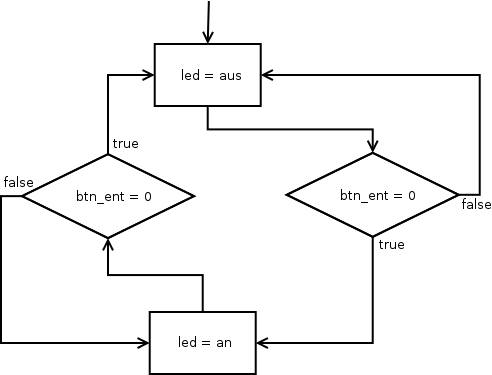
\includegraphics[width=0.7\textwidth]{\Path/resources/04-led.png}
	
	\paragraph{Entprellung} enthält die Komponente Zaehler, der bei der Veränderung des Eingangsignals gestartet wird und für 3ms weitere Änderungen ignoriert. (\ref{lst:04-entprellung}~Entprellung.vhdl-Code) \\
	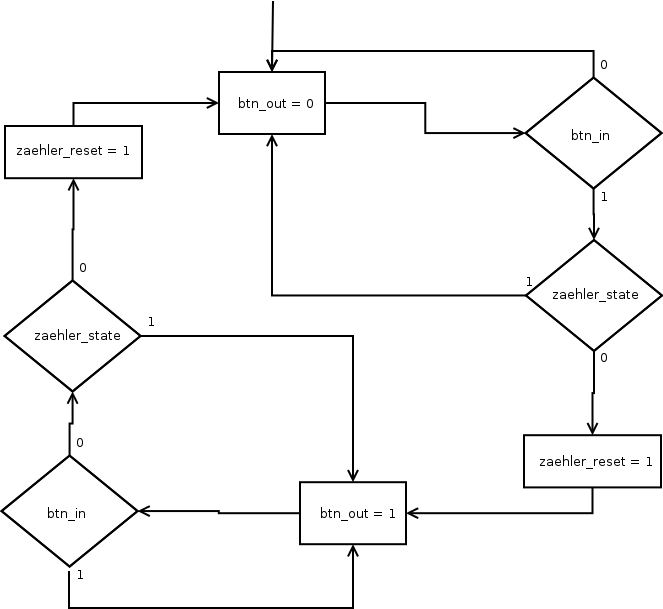
\includegraphics[width=0.8\textwidth]{\Path/resources/04-entpreller.png}


	\paragraph{Zaehler} implementiert einen Zähler, der durch ein Signal definierte Schritte zählt. Ausgegeben wird der aktuelle Zustand des Zählers. Eingegeben ein Reset-Signal. (\ref{lst:04-zaehler}~Zaehler.vhdl-Code) 
	\paragraph{Kopplung} \hfill\\
	Es wird eine synchrone Automatenkopplung über die Ausgangssignale mit einem Taktsignal verwendet.


\subsection{Auswertung}
	\paragraph{Ressourcenbedarf}
	\begin{itemize} 
	\item 86 Logik-Elemente
	\item davon 79 dedizierte Logik-Elemente
	\item 44 Register
	\item 3 Pins 
	\item maximale Taktfrequenz von 178 MHz
	\end{itemize}

%\endgroup
%	
%\newpage
%\section{Anhang}
\subsection{Circuit}
\label{lst:circuit}
\lstinputlisting[caption={Circuit.h}, language=C++]{\Path/../Simulator/src/main/Circuit.h}

\subsection{Simulator}
\label{lst:simulator}
\lstinputlisting[caption={Simulator.h}, language=C++]{\Path/../Simulator/src/main/Simulator.h}

\subsection{Solver}
\label{lst:solver}
\lstinputlisting[caption={Solver.h}, language=C++]{\Path/../Simulator/src/main/Solver.h}

\subsection{Parsers}
\label{lst:parsers}
\lstinputlisting[caption={Parsers.h}, language=C++]{\Path/../Simulator/src/parser/Parsers.h}

\subsection{Parser}
\label{lst:parser}
\lstinputlisting[caption={Parser.h}, language=C++]{\Path/../Simulator/src/parser/Parser.h}

\subsection{BENCH}
\label{lst:bench}
\lstinputlisting[caption={BENCH.h}, language=C++]{\Path/../Simulator/src/parser/BENCH.h}

\subsection{Gates}
\label{lst:gates}
\lstinputlisting[caption={Gates.h}, language=C++]{\Path/../Simulator/src/gates/Gates.h}

\subsection{Gate}
\label{lst:gate}
\lstinputlisting[caption={Gate.h}, language=C++]{\Path/../Simulator/src/gates/Gate.h}

\subsection{Input}
\label{lst:input}
\lstinputlisting[caption={Input.h}, language=C++]{\Path/../Simulator/src/gates/Input.h}

\subsection{DFF}
\label{lst:dff}
\lstinputlisting[caption={DFF.h}, language=C++]{\Path/../Simulator/src/gates/DFF.h}

\subsection{Output}
\label{lst:output}
\lstinputlisting[caption={Output.h}, language=C++]{\Path/../Simulator/src/gates/Output.h}
\newpage



\end{document}
